\documentclass[margin=0px]{article}

\usepackage{listings}
\usepackage[utf8]{inputenc}
\usepackage{graphicx}
\usepackage{float}
\usepackage[a4paper, margin=0.7in]{geometry}
\usepackage{amsthm}
\usepackage{fancyhdr}
\usepackage{setspace}

\onehalfspacing

\renewcommand{\figurename}{ábra}
\newenvironment{tetel}[1]{\paragraph{#1 \\}}{}

\pagestyle{fancy}
\lhead{\it{PTI BSc Záróvizsga tételek}}
\rhead{9. Objektumelvű tervezés}

\title{\textbf{{\Large ELTE IK - Programtervező Informatikus BSc} \vspace{0.2cm} \\ {\huge Záróvizsga tételek}} \vspace{0.3cm} \\ 9. Objektumelvű tervezés}
\author{}
\date{}

\begin{document}
\maketitle

\begin{tetel}{Objektumelvű tervezés}
    Nagy rendszerek fejlesztési fázisai, fejlesztési módszerek. SOLID tervezési elvek. Architekturális minták (MV, MVC stb.). Tervezési minták szerepe, osztályozása (létrehozási, szerkezeti, viselkedési), és kategóriánként 2-2 nevezetes tervezési minta bemutatása.
\end{tetel}

\section{Nagy rendszerek fejlesztési fázisai, kapcsolataik}

\subsection{Fejlesztési fázisok}
\begin{enumerate}
    \item A probléma megoldásának előzménye

          Egy probléma megoldása előtt meg kell vizsgálni a megvalósíthatóságát, és annak mikéntjét. Eredmény: \textit{Megvalósíthatósági tanulmány}, mely a következőkre válaszol:
          \begin{itemize}
              \item Erőforrások (hardver, szoftver, szakember)
              \item Költségek
              \item Határidő
              \item Üzemeltetés
          \end{itemize}
    \item Követelmények leírása

          Rendszerint iteratív módon állítjuk elő, és a prototípust használjuk a finomításra (ábra \ref{fig:kovetelmenyleiras}).

          \begin{figure}[H]
              \centering
              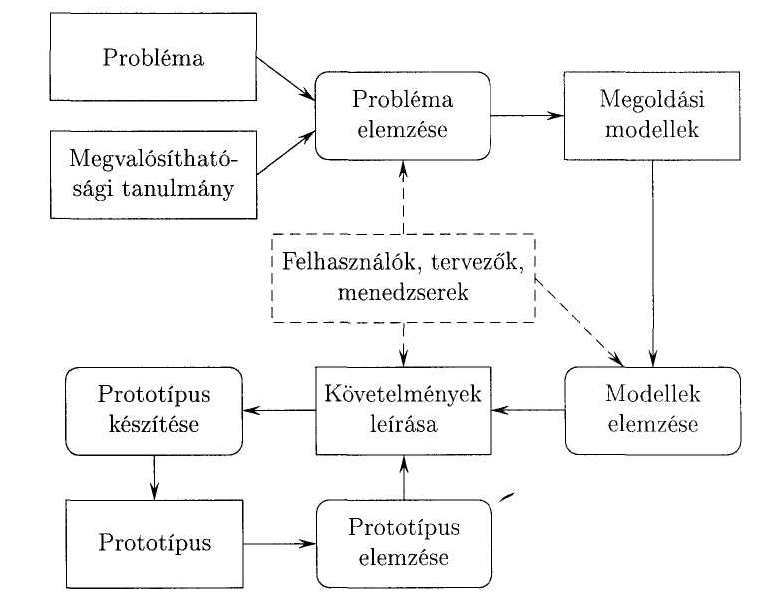
\includegraphics[width=0.5\textwidth]{img/kovetelmenyleiras.png}
              \caption{Követelményleírás elkészítésének folyamata}
              \label{fig:kovetelmenyleiras}
          \end{figure}

          Követelmények leírásának tartalma:

          \begin{itemize}
              \item Probléma
              \item Korlátozó tényezők (hardver, szoftver, stb.)
              \item Elfogadható megoldás
          \end{itemize}

          Követelmények leírásának fajtái:

          \begin{itemize}
              \item Funkcionális követelmények

                    A rendszer szolgáltatásainak, leképzéseinek leírása:
                    \begin{itemize}
                        \item Elindítás formája
                        \item Bemenő adatok (és azok megadásának formája)
                        \item Igénybevétel előfeltétele, korlátozások
                        \item Szolgáltatás kezdeményezésére a válasz, eredmények
                        \item Válasz megjelenési formája
                        \item Bemenő adatok és válasz közti reláció
                    \end{itemize}
              \item Nem funkcionális követelmények

                    A nem funkcionális követelményeket rendszerint három osztályba soroljuk: a termék követelményei, menedzselési követelmények, külső követelmények. Az osztályokat tovább lehet bontani (ábra \ref{fig:nemfunkckov}).
                    \begin{figure}[H]
                        \centering
                        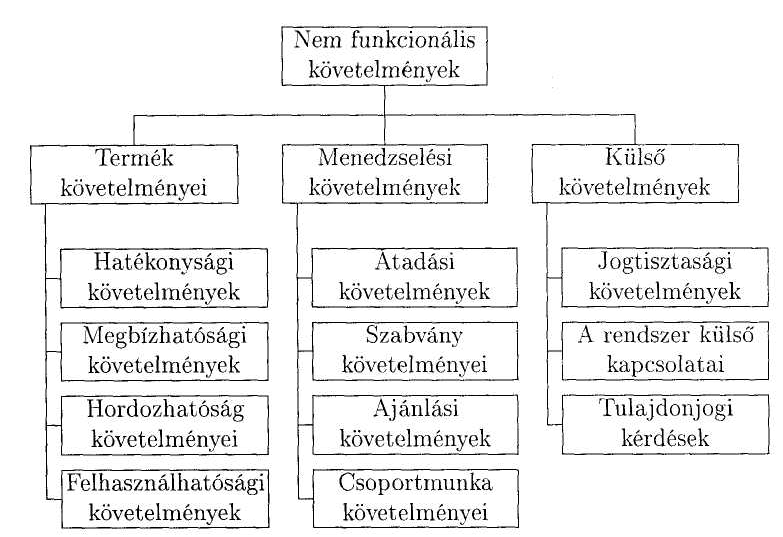
\includegraphics[width=0.5\textwidth]{img/nemfunkckov.png}
                        \caption{Nem funkcionális követelmények osztályozása}
                        \label{fig:nemfunkckov}
                    \end{figure}
          \end{itemize}

    \item Követelmények elemzése és prototípus

          A következőket kell megvizsgálni:
          \begin{itemize}
              \item Önmagában jó-e a követelmények leírása?
                    \begin{itemize}
                        \item Konzisztens (nincs ellentmondás)
                        \item Komplett (teljes)
                    \end{itemize}
              \item Validáció vizsgálat

                    (Megfelel-e a felhasználó által elképzelt problémának?)

              \item Megvalósíthatósági vizsgálat

                    (A követelményeknek megfelelő megoldás megvalósítható-e?)

              \item Tesztelhetőségi vizsgálat

                    (A követelmények úgy vannak-e megfogalmazva, hogy azok tesztelhetők?)

              \item Nyíltság kritériumainak vizsgálata.

                    (A követelmények nem mondanak-e ellent a módosíthatóság, a továbbfejleszthetőség
                    követelményének?)
          \end{itemize}

          A követelmények elemzésének egyik eszköze a prototípus-készítés.
          A prototípus magas szintű programozási környezetben létrehozott, a
          külső viselkedés szempontjából helyes megoldása a problémának.
    \item Programspecifikáció

          A programspecifikáció a következő kérdésekre kell, hogy válaszoljon a
          követelmények leírása alapján:

          \begin{itemize}
              \item Mik a bemenő adatok? (Forma, jelentés, megjelenés.)
              \item Mik az eredmények? (Forma, jelentés, megjelenés.)
              \item Mi a reláció a bemenő adatok és az eredmény adatok között?
          \end{itemize}
    \item Tervezés

          A tervezés során a következő kérdésekre adjuk
          meg a választ:
          \begin{enumerate}
              \item Statikus modell
                    \begin{itemize}
                        \item Rendszer szerkezete
                        \item Programegységek, azok feladata és kapcsolata
                    \end{itemize}
              \item Dinamikus modell
                    \begin{itemize}
                        \item Hogyan oldja meg a rendszer a problémát?
                        \item Milyen egységek működnek együtt?
                        \item Milyen üzenetek játszódnak le?
                        \item Rendszer és egységek állapotai
                        \item Események (melyek hatására állapotváltás történik)
                    \end{itemize}

              \item Funkcionális modell
                    \begin{itemize}
                        \item Milyen adatáramlások révén valósulnak meg a szolgáltatások?
                        \item Milyen leképezések játszanak szerepet az adatáramlásokban?
                        \item Mik az ajánlások az implementáció számára?
                              \begin{itemize}
                                  \item Implementációs stratégiára vonatkozó ajánlás.
                                  \item Programozási nyelvre vonatkozó előírás, ajánlás.
                                  \item Tesztelési stratégiára vonatkozó ajánlás.
                              \end{itemize}
                    \end{itemize}
          \end{enumerate}

          A gyakorlatban két tervezési módszer terjedt el:
          \textit{procedurális} és a \textit{objektumelvű}

          (\textit{procedurális}: megvalósítandó funkciókból, műveletekből indulunk ki, és ezek alapján bontjuk fel a rendszert kisebb összetevőkre, modulokra\\
          \textit{objektumelvű}: a rendszer funkciói helyett az
          adatokat állítjuk a tervezés középpontjába. A rendszer által használt
          adatok felelnek meg majd bizonyos értelemben az objektumoknak.)

    \item Implementáció

          Fontos szempontok:
          \begin{itemize}
              \item Reprezentáció (Adatok ábrázolása)
              \item Események leképezések megvalósítása

                    Algoritmusok és optimalizálások
          \end{itemize}

          Az implementáció egyik alapvető kérdése az implementációs stílus.
          A jó programozási stílus néhány fontos eleme:
          \begin{itemize}
              \item absztrakció különböző szintjeinek alkalmazása
              \item öröklődési technika használata, absztrakciós szintek hierarchikus
                    rendszere
              \item absztrakciós szintekre bontás osztályon belül (deklaráció + megvalósítás)
              \item korlátolt láthatóság;
              \item információ elrejtés (information hiding);
              \item információ beburkolás (encapsulation).
          \end{itemize}

    \item Verifikáció, validáció

          A rendszer eleget tesz-e a vele szemben támasztott elvárásoknak?

          Verifikáció: a specifikációszerinti helyesség igazolása

          Validáció: Minőségi előírások teljesítése (robosztusság hatékonyság, erőforrásigény)

          Ennek folyamata: tesztelés, melynek szakaszai:
          \begin{itemize}
              \item Egységteszt
              \item Rendszerteszt
          \end{itemize}
          A tesztelésnek két módja lehet:
          \begin{itemize}
              \item fekete doboz - Csak a maguknak a hibáknak a felderítése
              \item fehér doboz - Hibák helyének felderítése
          \end{itemize}

    \item Rendszerkövetés és karbantartás (maintenance)

          Karbantartás: Üzemebe helyezés után szükségessé váló szoftver jellegű munkák [pl.: rejtett hibák kijavítása, adaptációs munkák (új harver-, szoftverkörnyezet), továbbfejlesztési munkák]

          Rendszerkövetés: a felhasználókkal való kapcsolattartás menedzsment jellegű, dokumentációs feladatai [pl.: konfigurációk nyilvántartása, verziók menedzselése, dokumentáció menedzselése]

    \item Dokumentáció

          Egy nagy méretű program önmagában nem tekinthető szoftverterméknek
          dokumentáció nélkül. Egy jó dokumentáció a következőképp épül fel.
          \begin{itemize}
              \item Felhasználói leírás
                    \begin{itemize}
                        \item Feladatleírás
                        \item Futtató környezet
                        \item Fejlesztések, verziók
                        \item Installálás
                        \item Használat
                        \item Készítők
                    \end{itemize}
              \item Fejlesztői leírás
                    \begin{itemize}
                        \item Modulok (és azok szerkezete)
                        \item Osztályok (és azok kapcsolata)
                        \item Rendszer dinamikus viselkedése
                        \item Osztályok implementálása (adatszerkezetek, sablon osztályok)
                        \item Tesztelés
                    \end{itemize}
          \end{itemize}
\end{enumerate}

\subsection{Fejlesztési fázisok kapcsolatai}

A fejlesztési fázisok leírására többféle modellt használhatunk
\begin{enumerate}
    \item Vízesés modell

          Az egyes fázisok egymást követik, a
          módosítások a futtatási eredmények ismeretében történnek. Egy bizonyos
          fázisban elvégzett módosítás az összes rákövetkező fázist is érinti.

          \begin{figure}[H]
              \centering
              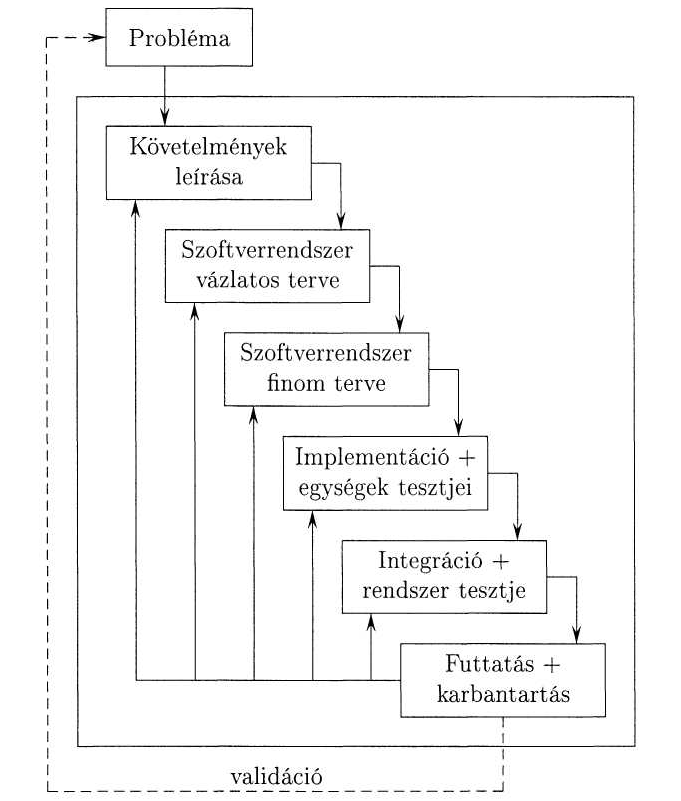
\includegraphics[width=0.5\textwidth]{img/vizeses.png}
              \caption{Vízesés modell}
              \label{fig:vizeses}
          \end{figure}

          Hárányai:
          \begin{itemize}
              \item Új szolgáltatás minden fázison módosítást igényel
              \item Validáció az egész életciklus megismétlését követelheti meg
          \end{itemize}
    \item Evolúciós modell

          A megoldást közelítő verzióinak, prototípusainak sorozatát
          állítjuk egymás után elő, és így haladunk lépésenként egészen a végleges
          megoldásig. Ennek során egy verzió elkészítésekor a specifikáció, a fejlesztés és a validáció párhuzamosan történik.

          \begin{figure}[H]
              \centering
              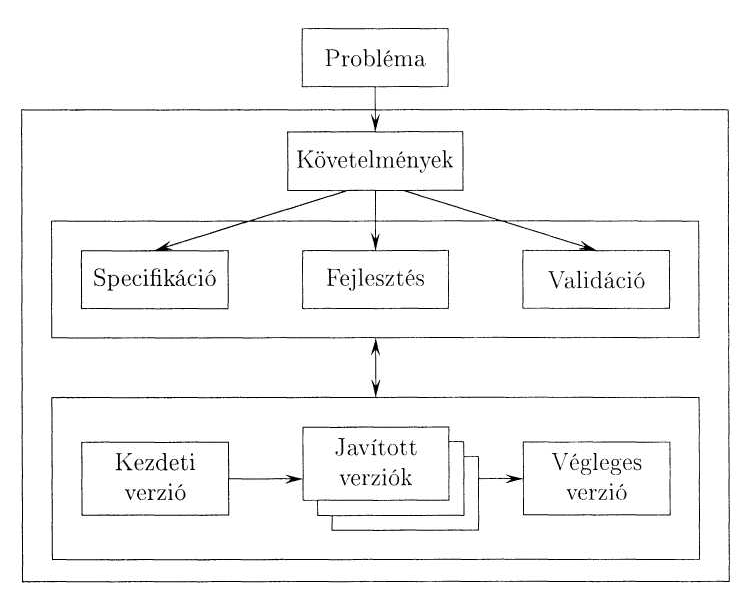
\includegraphics[width=0.5\textwidth]{img/evolucios.png}
              \caption{Evolúciós modell}
              \label{fig:evolucios}
          \end{figure}

          Hárányai:
          \begin{itemize}
              \item Nehéz a projekt áttekintése
              \item A gyors fejlesztés rendszerint a dokumentáltság rovására megy.
          \end{itemize}
    \item Boehm-féle spirális modell

          Ez a modell egy iterációs modell. Az iteráció a spirális egy
          fázisával modellezhető, amely négy szakaszra bontható:
          \begin{enumerate}
              \item Célok, utak, alternatívák, korlátozások definiálása
              \item Kockázatelemzés, stratégia kidolgozás
              \item Feladat megoldása, validáció
              \item Következő iteráció megtervezése
          \end{enumerate}

          \begin{figure}[H]
              \centering
              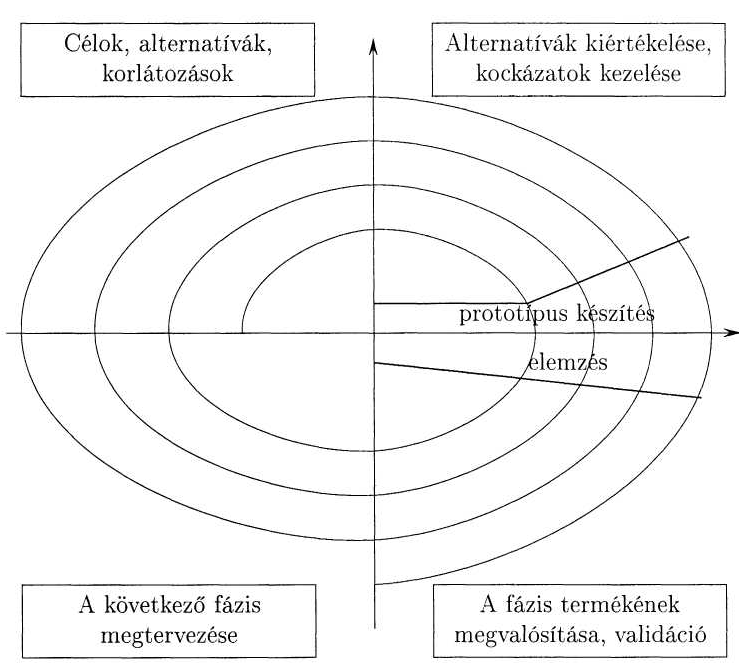
\includegraphics[width=0.4\textwidth]{img/spiral.png}
              \caption{Evolúciós modell}
              \label{fig:spiral}
          \end{figure}

          Hárányai:
          \begin{itemize}
              \item A modell alkalmazása általában munkaigényes, bonyolult feladat.
              \item A projekt kidolgozásához szükséges szakembereket nem könnyű
                    gazdaságosan foglalkoztatni.
          \end{itemize}
\end{enumerate}

\section{SOLID tervezési elvek}
Az objektumorientált programozásban a SOLID egy mozaikszó, amely az öt tervezési alapelv (Single responsibility principle, Open/closed principle, Liskov substitution principle, Interface segregation principle, Dependency inversion principle) kezdőbetűjéből áll, és célja, hogy a szoftvertervezést még érthetőbbé, rugalmasabbá és karbantarthatóbbá tegye. A SOLID-nak semmi köze a felelősségek hozzárendelésének általános mintáihoz (General Responsibility Assignment Software Patterns, GRASP). A S.O.L.I.D. alapelvek szülőatyja Robert Cecil Martin amerikai mérnök informatikus és tanácsadó, aki nem csak a ``tiszta kód mozgalom'' vezérszónoka, hanem többek között az Agile Manifesto egyik eredeti megfogalmazója is. Ezek az alapelvek adják a magját az agilis szoftverfejlesztésnek vagy adaptív szoftverfejlesztésnek. Az elméletét Martin Design Principles and Design Patterns című könyvében mutatta be, de mint mozaikszó csak később Michael Feathers révén terjedt el.

\begin{itemize}
    \item {\textbf {Egyetlen felelősség elve - Single Responsibility Principle}} Egy osztály vagy modul egy, és csak egy felelősséggel rendelkezzen (azaz: egy oka legyen a változásra).
    \item {\textbf {Nyílt/zárt elv - Open/Closed Principle}} Egy osztály vagy modul legyen nyílt a kiterjesztésre, de zárt a módosításra.
    \item {\textbf {Liskov helyettesítési elv - Liskov substitution principle}} Minden osztály legyen helyettesíthető a leszármazott osztályával anélkül, hogy a program helyes működése megváltozna.
    \item {\textbf {Interfész elválasztási elv - Interface segregation principle}} Az interfészek (kapcsolódási felületek) szétválasztásának elve: egyetlen kliens se legyen rákényszerítve arra, hogy olyan eljárásoktól függjön, amelyeket nem is használ.
    \item {\textbf {Függőség megfordítási elv - Dependency inversion principle}} A magas szintű modulok ne függjenek az alacsony szintű moduloktól. Mindkettő absztrakcióktól függjön.
\end{itemize}

\section{Architekturális minták (MV, MVC stb.)}

\subsection{MVC}
A modell-nézet-vezérlő (MNV) (angolul model-view-controller) a szoftvertervezésben használatos programtervezési minta. Összetett, sok adatot a felhasználó elé táró számítógépes alkalmazásokban gyakori fejlesztői kívánalom az adathoz (modell) és a felhasználói felülethez (nézet) tartozó dolgok szétválasztása, hogy a felhasználói felület ne befolyásolja az adatkezelést, és az adatok átszervezhetők legyenek a felhasználói felület változtatása nélkül. A modell-nézet-vezérlő ezt úgy éri el, hogy elkülöníti az adatok elérését és az üzleti logikát az adatok megjelenítésétől és a felhasználói interakciótól egy közbülső összetevő, a vezérlő bevezetésével.

Hagyományosan asztali felhasználói felületekhez használt, de manapság már webalkalmazásokhoz is népszerűvé vált. Népszerű programozási nyelvek mint a JavaScript, Python, Ruby, PHP, Java már külön telepítés szükségessége nélkül rendelkeznek MNV keretrendszerekkel web- és mobilalkalmazások fejlesztésére.

Gyakori egy alkalmazás több rétegre való felbontása: megjelenítés (felhasználói felület), tartománylogika és adatelérés. Az MNV-ben a megjelenítés tovább bomlik nézetre és vezérlőre. Az MNV sokkal inkább meghatározza egy alkalmazás szerkezetét, mint az egy programtervezési mintára jellemző.
\begin{description}
    \item[Modell (Model)] \hfill \\
        Az alkalmazás által kezelt információk tartomány-specifikus ábrázolása. A tartománylogika jelentést ad a puszta adatnak (pl. kiszámolja, hogy a mai nap a felhasználó születésnapja-e, vagy az összeget, adókat és szállítási költségeket egy vásárlói kosár elemeihez).

        Sok alkalmazás használ állandó tároló eljárásokat (mint mondjuk egy adatbázis) adatok tárolásához. Az MNV nem említi külön az adatelérési réteget, mert ezt beleérti a modellbe.
    \item[Nézet (View)] \hfill \\
        Megjeleníti a modellt egy megfelelő alakban, mely alkalmas a felhasználói interakcióra, jellemzően egy felhasználói felületi elem képében. Különböző célokra különböző nézetek létezhetnek ugyanahhoz a modellhez.
    \item[Vezérlő (Controller)] \hfill \\
        Az eseményeket, jellemzően felhasználói műveleteket dolgozza fel és válaszol rájuk, illetve a modellben történő változásokat is kiválthat.[8]
\end{description}

Az MNV gyakran látható webalkalmazásokban, ahol a nézet az aktuális HTML oldal, a vezérlő pedig a kód, ami összegyűjti a dinamikus adatokat és létrehozza a HTML-ben a tartalmat. Végül a modellt a tartalom képviseli, ami általában adatbázisban vagy XML állományokban van tárolva.

Habár az MNV-nek sok értelmezése létezik, a vezérlés menete általánosságban a következőképp működik:[9]
\begin{itemize}
    \item A felhasználó valamilyen hatást gyakorol a felhasználói felületre (pl. megnyom egy gombot).
    \item A vezérlő átveszi a bejövő eseményt a felhasználói felülettől, gyakran egy bejegyzett eseménykezelő vagy visszahívás útján.
    \item A vezérlő kapcsolatot teremt a modellel, esetleg frissíti azt a felhasználó tevékenységének megfelelő módon (pl. a vezérlő frissíti a felhasználó kosarát). Az összetett vezérlőket gyakran alakítják ki az utasítás mintának megfelelően, a műveletek egységbezárásáért és a bővítés egyszerűsítéséért.
    \item A nézet (közvetve) a modell alapján megfelelő felhasználói felületet hoz létre (pl. a nézet hozza létre a kosár tartalmát felsoroló képernyőt). A nézet a modellből nyeri az adatait. A modellnek nincs közvetlen tudomása a nézetről.
    \item A felhasználói felület újabb eseményre vár, mely az elejéről kezdi a kört.
\end{itemize}

A modell és a nézet kettéválasztásával az MNV csökkenti a szerkezeti bonyolultságot, és megnöveli a rugalmasságot és a felhasználhatóságot.

\begin{description}
    \item[Szolgáltatás (Service)] \hfill \\
        A vezérlő és a modell közötti réteg. A modelltől kér le adatokat és a vezérlőnek adja azt. Ennek a rétegnek a segítségével az adat tárolás (modell), adat lekérés (szolgáltatás) és a adat kezelés (vezérlő) elkülöníthetőek egymástól. Mivel ez a réteg nem része az eredeti MNV mintának, ezért használata nem kötelező.
\end{description}

\begin{description}
    \item[Előnyök:] \hfill
        \begin{itemize}
            \item Egyidejű fejlesztés – Több fejlesztő tud egyszerre külön a modellen, vezérlőn és a nézeteken dolgozni.
            \item Magas szintű összetartás – MNV segítségével az összetartozó funkciók egy vezérlőben csoportosíthatóak. Egy bizonyos modell nézetei is csoportosíthatóak.
            \item Függetlenség – MNV mintában az elemek alapvetően nagy részben függetlenek egymástól
            \item Könnyen változtatható – Mivel a felelősségek szét vannak választva a jövőbeli fejlesztések könnyebbek lesznek
            \item Több nézet egy modellhez – Modelleknek több nézetük is lehet
            \item Tesztelhetőség - mivel a felelősségek tisztán szét vannak választva, a külön elemek könnyebben tesztelhetőek egymástól függetlenül
        \end{itemize}
    \item[Hátrányok:] \hfill \\
        A MNV hátrányait általában a szükséges extra kódból adódnak.
        \begin{itemize}
            \item Kód olvashatósága – A keretrendszer új rétegeket add a kódhoz ami megnöveli a bonyolultságát
            \item Sok boilerplate kód – Mivel a programkód 3 részre bomlik a ebből az egyik fogja a legtöbb munkát végezni a másik kettő pedig az MNV minta kielégítése miatt létezik.'
            \item Nehezebben tanulható – A fejlesztőnek több különböző technológiát is ismernie kell a MNV használatához.
        \end{itemize}
\end{description}

\section{Tervezési minták szerepe, osztályozása, és kategóriánként 2-2 nevezetes tervezési minta bemutatása.}
Az informatikában a programtervezési mintának (angolul Software Design Patterns) nevezik a gyakran előforduló programozási feladatokra adható általános, újrafelhasználható megoldásokat. Egy programtervezési minta rendszerint egymással együttműködő objektumok és osztályok leírása.

A tervminták nem nyújtanak kész tervet, amit közvetlenül le lehet kódolni, habár vannak hozzájuk példakódok, amiket azonban meg kell tölteni az adott helyzetre alkalmas kóddal. Céljuk az, hogy leírást vagy sablont nyújtsanak. Segítik formalizálni a megoldást.

A minták rendszerint osztályok és objektumok közötti kapcsolatokat mutatnak, de nem specifikálják konkrétan a végleges osztályokat vagy objektumokat. A modellek absztrakt osztályai helyett egyes esetekben interfészek is használhatók, habár azokat maga a tervminta nem mutatja. Egyes nyelvek beépítetten tartalmaznak tervmintákat. A tervminták tekinthetők a strukturált programozás egyik szintjének a paradigma és az algoritmus között.

A legtöbb tervminta objektumorientált környezetre van kidolgozva. Mivel a funkcionális programozás kevéssé ismert és használt, arra a környezetre még csak kevés tervminta ismert, például a monád. Az objektumorientált minták közül nem mindegyiket lehet, és nem mindegyiket érdemes itt használni. Van, amit módosítani kell.

A programtervezési minták a 90-es évek elején (1994) tettek szert népszerűségre, amikor a négyek bandájaként vagy gammáékként (angolul "Gang of Four" vagy GoF)-ként emlegetett Erich Gamma, Richard Helm, Ralph Johnson és John Vlissides programozó négyes kiadta a Programtervezési minták című könyvüket, amely ma is alapjául szolgál az objektumorientált programozási minták kutatásának. Magát a tervmintát nem definiálták. A fogalom maga évekig formalizálatlan maradt.

Ez a könyv összesen 23 mintát mutat be, és a következő kategóriákba sorolja őket:
\begin{itemize}
    \item létrehozási minta
    \item szerkezeti minta
    \item viselkedési minta
\end{itemize}

A programtervezési minták a GoF definíciója szerint: egymással együttműködő objektumok és osztályok leírásai, amelyek testre szabott formában valamilyen általános tervezési problémát oldanak meg egy bizonyos összefüggésben. A szoftvertervezésben egy-egy problémára végtelen sok különböző megoldás adható, azonban ezek között kevés optimális van. Tapasztalt szoftvertervezők, akik már sok hasonló problémával találkoztak, könnyen előhúzhatnak egy olyan megoldást, amely már kipróbált és bizonyított. Kezdő fejlesztőknek viszont jól jön, ha mindazt a tudást és tapasztalatot, amit csak évek munkájával érhetnek el, precízen dokumentálva kézbe vehetik, tanulhatnak belőle és az általa bevezetett kifejezésekkel könnyebben beszélhetik meg egymás között az ötleteiket. A programtervezési minták ilyen összegyűjtött tapasztalatok, amelyek mindegyike egy-egy gyakran előforduló problémára ad általánosított választ. Azonban mindezek mellett még számos előnyük van:

\begin{itemize}
    \item lerövidítik a tapasztalatszerzési időt. A programtervezési mintákat nem feltalálták, hanem a gyakran előforduló problémákra adott optimális válaszokat gyűjtötték össze, ezáltal olyan megoldásokat adtak, amelyekre előbb-utóbb a legtöbb fejlesztő magától is rájönne – csak esetleg jóval később. Természetesen nem kizárt, hogy léteznek jobb, hatékonyabb megoldások, és ritka amikor egy-egy mintát pontosan úgy lehet alkalmazni egy problémára, ahogy az a könyvekben le van írva, de mindenképpen érdemes megismerni őket, ha másért nem is, hogy elsajátíthassunk valamennyit a szerzők látásmódjából.
    \item lerövidítik a tervezési időt. Az összes minta jól dokumentált, könnyen újrafelhasználható, így ha egyszer alkalmazzuk őket, jó eséllyel egy hasonló problémánál újra eszünkbe fognak jutni az összes előnyükkel és hátrányukkal együtt. Így azonnal hatékony, rugalmas megoldást adhatunk és megkímélhetjük magunkat sok tervezéstől és esetleges újratervezéstől. Ráadásul a minták után található következmények rész elősegíti, hogy teljesebb képet kapjunk az alkalmazás hatásairól is.
    \item közös szótárat ad a fejlesztők kezébe. Ez megkönnyíti az egymás közti kommunikációt és a program dokumentálását is, hiszen könnyebb úgy beszélni egy probléma megoldásáról, ha van egy közös alap, ahonnan indulunk vagy amihez lehet hasonlítani az új terveket.
    \item magasabb szintű programozást tesz lehetővé. Mivel ezek a minták elterjedtségük miatt már kiállták nagyon sok programozó próbáját, feltehetőleg az optimális megoldást tartalmazzák a problémára.
\end{itemize}

A tervezési minták a modulokat és kapcsolataikat szervezik. Alacsonyabb szintűek, mint az architekturális minták, amelyek a teljes rendszer általános felépítését jellemzik.

Több különböző tervminta létezik, például:
\begin{itemize}
    \item Algoritmus stratégia minták
    \item Magas szintű stratégiák, amelyek leírják, hogyan kell algoritmust szervezni egy adott architektúrára.
    \item Számítástervezési minták
    \item A kulcsfontosságú számítások megkeresését célozzák.
    \item Végrehajtási minták
    \item A végrehajtás alacsonyabb szintjén címzésekkel, feladatok végrehajtásának szervezésével, optimalizálásával, szinkronizálásával foglalkozó minták.
    \item Implementációs stratégia minták
    \item A forráskód implementációjában támogatják a program szervezését, és a párhuzamos programozás számára fontos adatszerkezetek felépítését.
    \item Szerkezeti tervezési minták
    \item Az alkalmazás globális struktúrájával foglalkoznak.
\end{itemize}

A tervmintákat Gammáék eredetileg három kategóriába csoportosították: létrehozási minták, szerkezeti minták, és viselkedési minták, amihez használták a delegálás, az aggregálás, és a konzultáció fogalmát. Objektumorientált környezetben az öröklődés, polimorfizmus és az absztrakt ősosztály fogalmait is felhasználják, habár az absztrakt osztályok többnyire interfészek is lehetnek. Egyes szerzők elkülönítik az architekturális tervezési mintákat is, mint a modell-nézet-vezérlő.

\subsection{Létrehozási minták (Egyke, Prototípus)}

\subsubsection{Egyke (Singleton)}
Biztosítja, hogy az osztályból csak egy példány készül, és biztosít egy publikus hozzáférést ehhez a példányhoz.

Az egyke programtervezési minta olyan programtervezési minta, amely egy objektumra korlátozza egy osztály létrehozható példányainak számát. Gyakori, hogy egy osztályt úgy kell megírni, hogy csak egy példány lehet belőle. Ehhez jól kell ismerni az objektumorientált programozás alapelveit. Az osztályból példányt a konstruktorával lehet készíteni. Ha van publikus konstruktor az osztályban, akkor akárhány példány készíthető belőle, tehát publikus konstruktora nem lehet az egykének. De ha nincs konstruktor, akkor nem hozható létre a példány, amin keresztül hívhatnánk a metódusait. A megoldást az osztályszintű (statikus) metódusok jelentik. Ezeket akkor is lehet hívni, ha nincs példány. Az egykének tehát van egy osztályszintű metódusa (szerezPéldány, angolul getInstance), ami minden hívójának ugyanazt a példányt adja vissza. Természetesen ezt a példányt is létre kell hozni, ehhez privát konstruktort kell készíteni, amit a szerezPéldány az egyke osztály tagjaként meghívhat.

\subsubsection{Prototípus (Prototype)}
Meghatároz egy előzetes mintát az objektumok létrehozásához, és később ez kerül másolásra. Gyakran használjuk, ha az objektum pontos típusa csak futásidőben derül ki.

A prototípus tervezési minta fő technikája a klónozás. A klónozás feladata, hogy az eredeti objektummal megegyező objektumot hozzon létre. Erre az egyszerű értékadás nem alkalmas, mert azok csak az objektum referenciáját másolják, így a két referencia ugyanoda mutat. A klónozásnak két fajtája van: sekély klónozás (angolul: shallow copy) és mély klónozás (angolul: deep copy).

\subsection{Szerkezeti minták (Díszítő, Helyettes)}

\subsubsection{Díszítő (Decorator)}
Lehetővé teszi az absztrakció változtatása nélkül további funkciók, felelősségi körök dinamikus hozzáadását.

A díszítő minta az átlátszó csomagolás klasszikus példája. Klasszikus példája a karácsonyfa. Attól, hogy a karácsonyfára felteszek egy gömböt, az még karácsonyfa marad, azaz a díszítés átlátszó. Ezt úgy érjük el, hogy az objektum összetételben szereplő mindkét osztály ugyanazon őstől származik, azaz ugyanolyan típusúak. Ez azért hasznos, mert a díszítő elemek gyakran változnak, könnyen elképzelhető, hogy új díszt kell felvenni. Ha díszítő egy külön típus lenne, akkor a karácsonyfa feldolgozó algoritmusok esetleg bonyolultak lehetnek.

A díszítő mintánál egy absztrakt ősből indulunk ki. Ennek kétfajta gyermeke van, alap osztályok, amiket díszíteni lehet és díszítő osztályok. A karácsonyfa példa esetén az alap osztályok a különböző fenyőfák. A díszítő osztályokat általában egy absztrakt díszítő osztály alá szervezzük, de ez nem kötelező.

A díszítés során az ős minden metódusát implementálni kell, úgy hogy, a becsomagolt példány metódusát meghívjuk, illetve ahol ez szükséges, ott hozzáadjuk a plusz funkcionalitást. Kétféle díszítésről beszélhetünk:
\begin{itemize}
    \item Amikor a meglévő metódusok felelősségkörét bővítjük. Ilyen a karácsonyfás példa.
    \item Amikor új metódusokat is hozzáadunk a meglévőkhöz. Ilyen a Java adatfolyam (angolul: stream) kezelése, illetve a lenti kölcsönözhető jármű példa.
\end{itemize}

Mindkét esetben a példányosítás tipikusan így történik:

ŐsOsztály példány = new DíszítőN(…new Díszítő1( new AlapOsztály())…);

Mivel a csomagolás átlátszó, ezért akárhányszor becsomagolhatjuk a példányunkat, akár egy díszítővel kétszer is. Ez rendkívül dinamikus, könnyen bővíthető szerkezetet eredményez, amit öröklődéssel csak nagyon sok osztállyal lehetne megvalósítani.

Érdekes megfigyelni a minta UML ábráján, hogy a díszítő osztályból visszafelé mutat egy aggregáció az ős osztályra. Ez az adatbázis kezelés Alkalmazott - Főnök reláció megoldásához hasonlít, amikor az Alkalmazott tábla önmagával áll egy-több kapcsolatban, ahol a külső kulcs a főnök alkalmazott\_ID értékét tartalmazza.

\subsubsection{Helyettes (Proxy)}
Egy másik objektum elfedésére, helyettesítésére alkalmazott tervezési minta.

A helyettes (angolul: proxy) tervezési minta egy nagyon egyszerű kompozícióra ad példát, ami ráadásul átlátszó becsomagolás. Egy valamilyen szempontból érdekes (drága, távoli, biztonsági szempontból érzékeny, …) példányt birtokol a helyettese. Ez az érdekes objektum nem érhető el kívülről, csak a helyettesén keresztül érhetők el a szolgáltatásai. Ugyanakkor a külvilág azt hiszi, hogy az érdekes objektumot közvetlenül éri el, mert a helyettes átlátszó módon csomagolja be az érdekes objektumot. Az átlátszóság miatt a helyettesnek és az érdekes objektumnak közös őse van.

Sokféle helyettes létezik aszerint, hogy milyen szempontból érdekes a helyettesített objektum, pl.:
\begin{itemize}
    \item Virtuális proxy: Nagy erőforrás igényű objektumok (pl. kép) helyettesítése a példányosítás (vagy más drága művelet) elhalasztásával, amíg ez lehetséges. A szövegszerkesztők ezt használják a képek betöltésére. Ha csak gyorsan átlapozom a dokumentumot, akkor a kép nem töltődik be (elhalasztódik a betöltés), csak helye látszik.
    \item Távoli proxy: Távoli objektumok lokális megjelenítése átlátszó módon. A kliens nem is érzékeli, hogy a tényleges objektum egy másik gépen van, amíg van hálózati kapcsolat. Ezt alkalmazza a távoli metódus hívás (remote method invocation – RMI).
    \item Védelmi proxy: A hozzáférést szabályozza különböző jogok esetén.
    \item Okos referencia: Az egyszerű referenciát helyettesíti olyan esetekben, amikor az objektum elérésekor további műveletek szükségesek.
    \item Gyorsító tár (cache): Ha van olyan számítás (ide sorolva a letöltéseket is), ami drága, akkor a számítás eredményét érdemes letárolni egy gyorsító tárban, ami szintén egyfajta proxy.
\end{itemize}

\subsection{Viselkedési minták (Állapot, Megfigyelő)}

\subsubsection{Állapot (State)}
Az objektum viselkedése megváltoztatható a belső állapottól függően.

Lehetővé teszi egy objektum viselkedésének megváltozását, amikor megváltozik az állapota. Példa: TCPConnection osztály egy hálózati kapcsolatot reprezentál; Három állapota lehet: Listening, Established, Closed; a kéréseket az állapotától függően kezeli.

Használjuk, ha
\begin{itemize}
    \item az objektum viselkedése függ az állapotától, és a viselkedését az aktuális állapotnak megfelelően futás közben meg kell változtatnia, illetve
    \item a műveleteknek nagy feltételes ágai vannak, melyek az objektum állapotától függenek.
\end{itemize}

Előnyök:
\begin{itemize}
    \item Egységbe zárja az állapotfüggő viselkedést, így könnyű új állapotok bevezetése.
    \item Áttekinthetőbb kód (nincs nagy switch-case szerkezet).
    \item A State objektumokat meg lehet osztani.
\end{itemize}

Hátrányok: Nő az osztályok száma (csak indokolt esetben használjuk).

\subsubsection{Megfigyelő (Observer)}
Meghatároz ez egy-a-többhöz függőséget objektumok között. Egy adott objektum módosulásáról automatikus értesítő információt küld a tőle függő objektumoknak, amik ezek alapján frissülnek.

ehetővé teszi, hogy egy objektum megváltozása esetén értesíteni tudjon tetszőleges más objektumokat anélkül, hogy bármit is tudna róluk. Részei:
\begin{itemize}
    \item Alany: Tárolja a beregisztrált megfigyelőket, interfészt kínál a megfigyelők be- és kiregisztrálására valamint értesítésére.
    \item Megfigyelő: Interfészt definiál azon objektumok számára, amelyek értesülni szeretnének az alanyban bekövetkezett változásról. Erre a frissít (update) metódus szolgál.
\end{itemize}

Két fajta megfigyelő megvalósítást ismerünk:
\begin{itemize}
    \item ``Pull-os'' megfigyelő: Ebben az esetben a megfigyelő lehúzza a változásokat az alanytól.
    \item ``Push-os'' megfigyelő: Ebben az esetben az alany odanyomja a változásokat a megfigyelőnek.
\end{itemize}

A kettő között ott van a különbség, hogy a frissít metódus milyen paramétert kap. Ha az alany átadja önmagát (egy frissít(this) hívás segítségével) a megfigyelőnek, akkor ezen a referencián keresztül a megfigyelő képes lekérdezni a változásokat. Azaz ez a ``pull-os'' megoldás.

Ha a frissít metódusnak az alany azokat a mezőit adja át, amik megváltoztak és amiket a megfigyelő figyel, akkor ``push-os'' megoldásról beszélünk. A következő példában épp egy ilyen megvalósítást láthatunk.

\end{document}